\documentclass[journal, onecolumn]{IEEEtran}
\IEEEoverridecommandlockouts
% The preceding line is only needed to identify funding in the first footnote. If that is unneeded, please comment it out.
\usepackage{cite}
\usepackage{amsmath,amssymb,amsfonts}
\usepackage{algorithmic}
\usepackage{textcomp}
\usepackage{theorem,caption,extarrows,mathrsfs}
\usepackage{graphicx,xcolor,hyperref,booktabs,float,subfig,overpic}
\usepackage{tikz}
\usepackage[european]{circuitikz}
\usetikzlibrary{calc}
\usepackage{pgfplots,grffile}
\usepackage{fontspec}
\usepackage[skins]{tcolorbox}
\setmainfont{STIX Two Text}
\setsansfont{CMU Sans Serif}
\setmonofont{Sarasa Fixed SC Nerd Font}
\pgfplotsset{compat=newest}
%% the following commands are needed for some matlab2tikz features
\usetikzlibrary{plotmarks}
\usetikzlibrary{arrows.meta}
\usetikzlibrary{calc}
\usepgfplotslibrary{patchplots}
\def\BibTeX{{\rm B\kern-.05em{\sc i\kern-.025em b}\kern-.08em
T\kern-.1667em\lower.7ex\hbox{E}\kern-.125emX}}
%% href setup
\usepackage[normalem]{ulem}
\definecolor{mylinkcolor}{HTML}{0078D4}
\definecolor{myulcolor}{HTML}{00487F}
\hypersetup{
	hidelinks=true
}
% \newcommand\reduline{\bgroup\markoverwith{\textcolor{red}{\rule[-0.5ex]{2pt}{0.4pt}}}\ULon}
\makeatletter
  \newcommand\reduline{\bgroup\markoverwith{\textcolor{red}{\rule[-0.5ex]{2pt}{0.4pt}}}\ULon}
  \UL@protected\def\bluedotuline{\leavevmode \bgroup
    \UL@setULdepth
    \ifx\UL@on\UL@onin \advance\ULdepth2\p@\fi
    \markoverwith{\begingroup
       %\advance\ULdepth0.08ex
       \lower\ULdepth\hbox{\kern.06em \textcolor{myulcolor}{.}\kern.04em}%
       \endgroup}%
    \ULon}
  \UL@protected\def\bluedashuline{\leavevmode \bgroup
    \UL@setULdepth
    \ifx\UL@on\UL@onin \advance\ULdepth2\p@\fi
    \markoverwith{\kern.13em
    \vtop{\color{myulcolor}\kern\ULdepth \hrule width .3em}%
    \kern.13em}\ULon}
\makeatother

\newcommand{\myhy}[1]{%
	\hyperref[#1]{\color{mylinkcolor}\bluedotuline{\textit{\ttfamily\footnotesize #1}}}%
}
%% Listings setup
\usepackage{listings}
\lstset{
    basicstyle          =   \sffamily,          % 基本代码风格
    keywordstyle        =   \bfseries,          % 关键字风格
    commentstyle        =   \rmfamily\itshape,  % 注释的风格,斜体
    stringstyle         =   \ttfamily,  % 字符串风格
    flexiblecolumns,                % 别问为什么,加上这个
    numbers             =   left,   % 行号的位置在左边
    showspaces          =   false,  % 是否显示空格,显示了有点乱,所以不现实了
    numberstyle         =   \tiny\ttfamily,    % 行号的样式,小五号,tt等宽字体
    showstringspaces    =   false,
    captionpos          =   t,      % 这段代码的名字所呈现的位置,t指的是top上面
    frame               =   shadowbox,   % 显示边框
    rulesepcolor=\color{red!20!green!20!blue!20}
}

\lstdefinestyle{Python}{
    language        =   Python, % 语言选Python
    backgroundcolor=\color{backpycol},
    basicstyle      =   \ttfamily,
    numberstyle     =   \ttfamily,
    keywordstyle    =   \color{blue},
    keywordstyle    =   [2] \color{teal},
    stringstyle     =   \color{magenta},
    commentstyle    =   \color[HTML]{338AAF}\ttfamily,
    breaklines      =   true,   % 自动换行,建议不要写太长的行
    columns         =   fixed,  % 如果不加这一句,字间距就不固定,很丑,必须加
    basewidth       =   0.5em,
}
\definecolor{codegreen}{rgb}{0,0.6,0}
\definecolor{codegray}{rgb}{0.5,0.5,0.5}
\definecolor{codepurple}{rgb}{0.58,0,0.82}
\definecolor{backcolour}{rgb}{0.95,0.95,0.92}
\definecolor{backpycol}{rgb}{0.97,0.95,0.97}
\lstdefinestyle{C++}{
    language =[ANSI]C,
    backgroundcolor=\color{backcolour},
    commentstyle=\color[HTML]{338AAF}\ttfamily,
    keywordstyle=\sffamily\bfseries\color{magenta},
    numberstyle=\color{codegray},
    stringstyle=\color{codepurple},
    basicstyle=\ttfamily,
    breakatwhitespace=false,
    breaklines=true,
    basewidth=0.5em,
    captionpos=b,
    columns=fixed,
    frame=shadowbox,
    keepspaces=true,
    numbers=left,
    numbersep=5pt,
    showspaces=false,
    showstringspaces=false,
    showtabs=false,
    tabsize=4
}
\lstdefinestyle{matlab}{
    language=matlab,
    backgroundcolor=\color{backcolour},
    commentstyle=\color[HTML]{338AAF}\ttfamily,
    keywordstyle=\sffamily\bfseries\color{magenta},
    numberstyle=\color{codegray},
    stringstyle=\color{codepurple},
    basicstyle=\ttfamily,
    breakatwhitespace=false,
    breaklines=true,
    basewidth=0.5em,
    captionpos=b,
    columns=fixed,
    keepspaces=true,
    numbers=left,
    numbersep=5pt,
    showspaces=false,
    showstringspaces=false,
    showtabs=false,
    tabsize=4,
    frame=shadowbox
}
\definecolor{mygreen}{rgb}{0,0.6,0}
\definecolor{mygray}{rgb}{0.5,0.5,0.5}
\definecolor{mymauve}{rgb}{0.58,0,0.82}
\definecolor{bggray}{rgb}{0.93,0.95,0.94}
\lstdefinestyle{pseudocode}{
    backgroundcolor=\color{bggray},
    columns=fullflexible,
    tabsize=4,
    breaklines=true,               % automatic line breaking only at whitespace
    captionpos=b,                  % sets the caption-position to bottom
    commentstyle=\color{mygreen},  % comment style
    escapeinside={\%*}{*)},        % if you want to add LaTeX within your code
    keywordstyle=\color{blue},     % keyword style
    stringstyle=\color{mymauve}\ttfamily,  % string literal style
    frame=shadowbox,
    rulesepcolor=\color{red!20!green!20!blue!20},
    % identifierstyle=\color{red},
    language=c++,
    numbers=left,
    numberstyle=\small\color{codegray},
    basicstyle=\ttfamily,% size of fonts used for the code
    escapeinside=``,
    xleftmargin=0.6em,
    xrightmargin=0.6em,
    aboveskip=1em
}
\lstdefinestyle{Fortran}{
    language =fortran,
    backgroundcolor=\color{backcolour},
    commentstyle=\color[HTML]{338AAF}\ttfamily,
    keywordstyle=\sffamily\bfseries\color{magenta},
    numberstyle=\small\color{codegray},
    stringstyle=\color{codepurple},
    basicstyle=\ttfamily,
    breakatwhitespace=false,
    breaklines=true,
    basewidth=0.5em,
    captionpos=b,
    columns=fixed,
    frame=shadowbox,
    keepspaces=true,
    numbers=left,
    numbersep=5pt,
    showspaces=false,
    showstringspaces=false,
    showtabs=false,
    tabsize=4
}

\title{EE332 Lab2: Divide-Conquer Implementation of 16-4 Priority Encoder}
\author{
	\IEEEauthorblockN{1\textsuperscript{st} Qiu Kunyuan}
	\IEEEauthorblockA{
		\textit{EEE. Southern University of Science and Technology}\\
		Shenzhen, PRC\\
		11913019@mail.sustech.edu.cn
	}
}
\begin{document}
\maketitle
% !TEX root=./report_lab2.tex

\begin{abstract}
	This report focuses on the difference between cascaded structure and tree structure in the Verilog implementation of 16-4 priority encoder. The timing optimization of combinational logic circuits with a large number of inputs is carried out by the divide and conquer method, and the pipelining method is also employed. Therefore, the routing results are obtained with satisfactory delays and no race-hazard jitters.

	Code for this experiment can be found at \myhy{https://github.com/KagaJiankui/EE332-2024S/tree/master/lab3/lab3.srcs}.
\end{abstract}
\vspace{1em}
\begin{IEEEkeywords}
	FPGA, programmable logic, priority coder, divide-conquer method, pipelining, -hazard condition, jitter, delay
\end{IEEEkeywords}

\section{Introduction}

There are typically two main implementations of priority encoders in Verilog designs: cascaded architecture and tree architecture.

\begin{itemize}
	\item \textbf{Cascaded architecture}: A cascaded architecture is a serial structure that groups input signals and encodes them within each group, and then these results are cascaded. Such a structure enjoys the simplicity of implementation, but suffers from the disadvantage that the delay increases with the increase in the number of input signals.
	\item \textbf{Tree architecture}: A tree architecture is a parallel structure that encodes all the input signals simultaneously. Benefit of this structure is its speed as all the operations are performed in parallel. However, the demerit of this structure is the requirement of more hardware resources.
\end{itemize}

\subsection{Cascaded Architecture}

The code of cascaded priority encoder is \lstinline{if-else} statements organized along with the order of MSB to LSB. Thus, the cascaded priority encoderan can be easily modeled by the following Verilog code with parameter \lstinline{digit}:

\begin{lstlisting}[language=verilog, style=verilog]
module encoder
  #(
    parameter digit=8
    parameter digit_output=3
  )
  (
    input  [digit-1:0] x
    input  en,
    output reg [digit_output-1:0]y
  );
  integer i;
  always @(x or en) begin
    if (en) begin
      y = 0;
      for( i = 0; i <= digit - 1; i = i+1)
          if(x[i] == 1)  y = i[digit-1:0];
    end
    else  y = 0;
  end
endmodule
\end{lstlisting}

For 8-3 encoder, the module is instantialized with parameter \lstinline{.digit(8), .digit_out(3)} that generates the following if-else statements,

\begin{lstlisting}[language=verilog,style=verilog]
module encoder (
  input [7:0] x,
  input en,
  output reg [2:0] y,
  output reg v
);
  always @ (x or en)
    if (x>0 & en==1) begin
      if (x[7]) y = 3'b111;
      else if (x[6]) y = 3'b110;
      else if (x[5]) y = 3'b101;
      else if (x[4]) y = 3'b100;
      else if (x[3]) y = 3'b011;
      else if (x[2]) y = 3'b010;
      else if (x[1]) y = 3'b001;
      else if (x[0]) y = 3'b000;
      else y = 3'b000;
    end
    else begin
      y = 0;
      v = 0;
  end
endmodule
\end{lstlisting}

and the schematic (\ref{cascaded_83_encoder}) of the elaboration result is basically directly translated from the HDL description, which are cascaded MUXs.

\begin{figure}[htpb]
	\begin{center}
		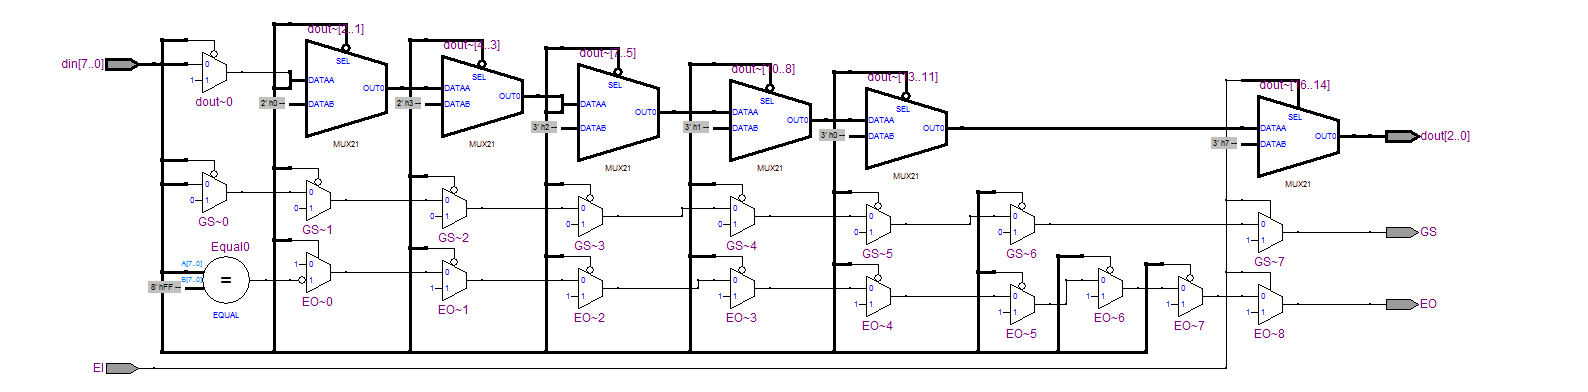
\includegraphics[width=0.98\textwidth]{report_lab3.assets/20240321191356.png}
		\caption{Synthesis result of parameterized 8-3 priority encoder}
		\label{cascaded_83_encoder}
	\end{center}
\end{figure}

For 4-2 encoder, the module is instantialized with parameter \lstinline{.digit(4), .digit_out(2)},

\lstinputlisting[language=verilog, style=verilog]{../../lab3/lab3.srcs/sources_1/new/encoder4x2_cas.v}

which is elaborated into similiar schematic (\ref{cascaded_42_encoder}):

\begin{figure}[htpb]
	\begin{center}
		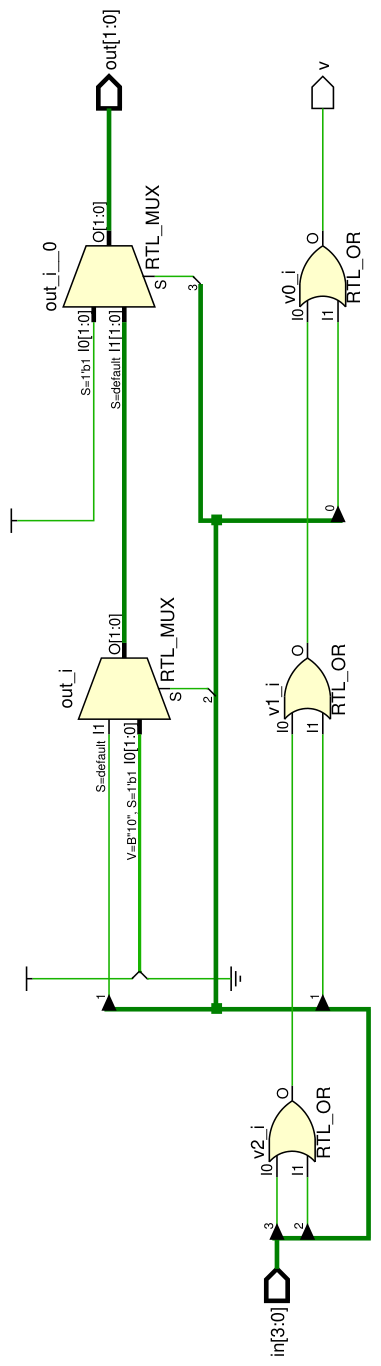
\includegraphics[height=0.80\textwidth, angle=270]{report_lab3.assets/encoder42_cas_elab.png}
		\caption{Synthesis result of parameterized 4-2 priority encoder}
		\label{cascaded_42_encoder}
	\end{center}
\end{figure}

\end{document}